%------------------------------------------------------------------------------%
%-                        1. 时间复杂度の比较                                                                            -%
%-                        2. 算法伸缩性の比较                                                                            -%
%-                        3. 图布局算法の细化                                                                            -%
%-                        4. 系统功能の补全、上传导出、分层导览视图                                -%
%------------------------------------------------------------------------------%
%- Copyright (C) Huangrui Mo <huangrui.mo@gmail.com>
%- This is free software: you can redistribute it and/or modify it
%- under the terms of the GNU General Public License as published by
%- the Free Software Foundation, either version 3 of the License, or
%- (at your option) any later version.
%---------------------------------------------------------------------------%
%->> Document class declaration
%---------------------------------------------------------------------------%
\documentclass[printcopy,fontset=fandol]{Style/neuthesis}%
%- Multiple optional arguments:
%-
%- [<singlesided|doublesided|printcopy>]% set one or two sided eprint or print
%- [draftversion]% show draft version information
%- [fontset=<fandol|windows|mac|adobe>]% specify font set to replace automatic detection
%- [scheme=plain]% thesis writing of international students
%- [standard options for ctex book class: draft|paper size|font size|...]%
%---------------------------------------------------------------------------%
%->> Document settings
%---------------------------------------------------------------------------%
\usepackage[bibtex,myhdr,table,list,geometry,url]{Style/artratex}

% document settings
%- usage: \usepackage[option1,option2,...,optionN]{artratex}
%- Multiple optional arguments:
%- [bibtex|biber]% set bibliography processor and package
%- [geometry]% reconfigure page layout via geometry package
%- [lscape]% provide landscape layout environment
%- [myhdr]% enable header and footer via fancyhdr package
%- [color]% provide color support via xcolor package
%- [background]% enable page background
%- [tikz]% provide complex diagrams via tikz package
%- [table]% provide complex tables via ctable package
%- [list]% provide enhanced list environments for algorithm and coding
%- [math]% enable some extra math packages
\usepackage{Style/artracom}% user defined commands
%---------------------------------------------------------------------------%
%->> Document inclusion
%---------------------------------------------------------------------------%
%\includeonly{Tex/Chap_1,...,Tex/Chap_N}% selected files compilation
%---------------------------------------------------------------------------%
%->> Document content
%---------------------------------------------------------------------------%
\def\alltex{}
\begin{document}
% \layout
%-
%-> Frontmatter: title page, abstract, content list, symbol list, preface
%-
\frontmatter% initialize the environment
% !TEX ROOT = ../Thesis.tex
%---------------------------------------------------------------------------%
%->> 封面信息及生成
%---------------------------------------------------------------------------%
%-
%-> 中文封面信息
%-
\category{}%分类号
\confidential{}% 密级:只有涉密论文才填写
\UDC{}
\schoollogo% 校徽
% \schooltitle{width=1cm}{neu_title}
\title{...deleted...}% 论文中文题目
\author{...deleted...}% 论文作者
\advisor{...deleted...}% 指导教师:姓名 专业技术职务 工作单位
\advisorsec{东北大学计算机科学与工程学院}% 指导老师附加信息 或 第二指导老师信息
\degree{硕士}% 学位:学士、硕士、博士
\degreetype{工学}% 学位类别:理学、工学、工程、医学等
\major{...deleted...}% 二级学科专业名称
\institute{...deleted...}% 院系名称

\research{...deleted...}% 研究方向
\authorno{...deleted...}% 学号
\chinesedate{2019~年~7~月}%  封面页脚日期
\submissiondate{2019~年~7~月}% 论文提交日期
\oraldefencedate{2019~年~7~月}% 论文答辩日期
\degreedate{2019~年~7~月}% 学位授予日期
\chairman{}% 答辩委员会主席
%-
%-> 英文封面信息
%-
\englishtitle{...deleted...}% 论文英文题目
\englishauthor{...deleted...}% 论文作者
\englishadvisor{...deleted...}% 指导教师
\englishdegree{Master}% 学位:Bachelor, Master, Doctor。封面格式将根据英文学位名称自动切换,请确保拼写准确无误
\englishdegreetype{Engineering}% 学位类别:Philosophy, Natural Science, Engineering, Economics, Agriculture 等
\englishthesistype{thesis}% 论文类型: thesis, dissertation
\englishuniversity{Northeastern University}
\englishmajor{Computer Thechnology}% 二级学科专业名称
\englishinstitute{School of Computer Science and Engineering}% 院系名称
\englishdate{June 2019}% 毕业日期:春季 April 夏季为June、秋季为September 冬季为December
%-
%-> 生成封面
%-
\makereviewcover % 生成盲审中文封面
\makeprintcover %生成打印的中文封面
\makechinesetitle % 生成中文内容页
\makeenglishtitle% 生成英文页
%-
%-> 作者声明
%-
\makedeclaration% 生成声明页
% title page, abstract, dedication
% !TEX ROOT = ../Thesis.tex
%-
%-> 中文摘要
%-
\chapter{摘\quad 要}\chaptermark{摘\quad 要}% 摘要标题
% \setcounter{page}{1}% 开始页码
% \pagenumbering{Roman}% 页码符号
% 22p / 12p = 1.83
\linespread{1.5}
\zihao{-4}
% \setlength{\baselineskip}{20pt}

信息可视化主要研究非数值型信息资源的视觉展示,以达到帮助人们理解并分析数据的目的。随着科技的不断发展,图亦或是网络在我们的生活中出现的越来越多,图数据的产生速度和存储规模也符合大数据时代的发展趋势。与此同时,这些复杂结构中蕴含的隐藏信息也越来越多,对这些网络的进行高效的分析、挖掘及视觉呈现一直是数据科学及可视化领域的研究热点。在这一背景下,诸如社交网络等传统的图数据达到了前所未有的规模,经典的单机可视化解决方案已经无法高效的对海量图数据进行展现,传统的基于数据处理的数据挖掘策略又很难直观的描述或解释其结果。因此迫切需要一种可以有效展现海量图数据的可视化解决方案,以达到在可容忍的时间内对大规模图数据进行直观、可解释的可视分析。如何缩短处理时间以及如何直观、有意义的对数据进行布局展现是一个十分具有挑战性的课题,这也是本文的主要研究内容。

在保证布局质量方面,本文首先分析了单机布局方案的局限性和各种已有分布式处理模型的特点。随后在分层抽样算法及K核分解思想的基础上,提出了面向大图的抽样算法,在尽可能保证抽样结构相似性的前提下对大规模图数据进行分层抽样,最终的实验证明,该方法在抽样结构的相似性上有着比SBS、SS等算法更好的表现,能够更好的保留原结构的拓扑信息。

在改善布局算法方面,本文通过将抽样方法应用到布局过程中,分层逐级对图数据进行显示。为此,本文实现了基于GraphX的力导向布局算法,并将其与上述分层抽样算法结合,由简入繁逐渐细化地对原结构进行布局及展示。在大规模数据处理的过程中,该方案能够有效减少计算需求,并且能够更加灵活的适应可视分析的需要。

最后,本文设计了大规模图数据可视化原型系统,基于GraphX实现分层布局算法,借助浏览器(B/S结构)实现整个可视化界面。并借助此系统对上述提出的抽样及布局算法进行了实验。与现有的单机系统相比,可以处理前者无法有效处理的大图数据;同时与已有的分布式可视化系统相比,可以赋予使用者更细粒度的视图控制能力并得到更清晰的结果展示。


\keywords{图数据抽样; 分层图布局; 分布式计算; K核分解}% 中文关键词
%-
%-> 英文摘要
%-
\chapter{Abstract}\chaptermark{Abstract}% 摘要标题

Information visualization mainly studies the visual display of non-numerical information resources in order to help people understand and analyze data. With the continuous development of science and technology, more and more graphs or networks appear in our lives. The speed and storage scale of graph data also conform to the development trend of the era of big data. At the same time, more and more hidden information is contained in these complex structures. Efficient analysis, mining and visual presentation of these networks has always been a research hotspot in the field of data science and visualization. In this context, traditional graph data such as social networks have reached an unprecedented scale. The classical single-machine visualization solution has been unable to effectively display large amounts of graph data. The traditional data mining strategy based on data processing is difficult to intuitively describe or explain the results. Therefore, there is an urgent need for a visualization solution that can effectively display massive graph data in order to achieve intuitive and interpretable visual analysis of large-scale graph data in tolerable time. How to shorten the processing time and how to visually and meaningfully display the layout of data is a very challenging topic, which is also the main research content of this thesis.

In order to ensure the layout quality, this thesis first analyses the limitations of the single-machine layout scheme and the characteristics of various existing distributed processing models. Subsequently, on the basis of hierarchical sampling algorithm and K-kernel decomposition idea, a large-scale graph-oriented sampling algorithm is proposed. On the premise of ensuring the similarity of sampling structure as much as possible, the large-scale graph data are stratified sampled. The final experiment proves that this method has better performance than other algorithms in the similarity of sampling structure, and can better retain the topological information of the original structure.

In order to improve the layout algorithm, the sampling method is applied to the layout process, and the graph data is displayed hierarchically and step by step. To this end, this thesis implements a force-oriented layout algorithm based on GraphX, and combines it with the above-mentioned hierarchical sampling algorithm, which gradually refines the layout and display of the original structure from simplicity to complexity. In the process of large-scale data processing, this scheme can effectively reduce the computational requirements and be more flexible to meet the needs of visual analysis.

Finally, this thesis designs a large-scale graphics data visualization prototype system, using GraphX to compute the coordinates of graph nodes, using B/S mode to achieve the entire visualization interface with the help of browser. With the help of this system, the sampling and layout algorithms proposed above are experimented. Compared with the existing single-machine system, it can deal with the large-scale map data which the former can not effectively handle; at the same time, compared with the existing distributed visualization system, it can give users more fine-grained view control ability and get clearer results display.

\englishkeywords{Graph sampling; Hierarchical layout; Distributed computing; K-core decomposition }
 % abstract (chinese and english)

{% content list region
% \linespread{1}
% \intotoc{\contentsname}% add link to contents table and bookmark
% \chapter*{\contentsname}
\linespread{1.25}% local line space
\tableofcontents% contents catalog

%硕士论文不需要表格和图片的索引
%\intotoc{\listfigurename}% add link to contents table and bookmark
%\listoffigures% figures catalog

%\intotoc{\listtablename}% add link to contents table and bookmark
%\listoftables% tables catalog
}
% \input{Tex/Prematter}% list of symbols, preface content
%-
%-> Mainmatter
%-
\mainmatter% initialize the environment
\linespread{1.5}
\zihao{-4}
%---------------------------------------------------------------------------%
%->> Main content
%---------------------------------------------------------------------------%
\chapter{绪论}\label{chap:绪论}

\section{研究背景}

    \subsection{图数据的产生和发展}

    ... deleted ...





    \subsection{图数据的可视化技术}

    ... deleted ...




\section{研究意义}

    \subsection{大规模图数据可视化的重要性}

    ... deleted ...

    \begin{itemize}
        \item ... deleted ...
        \item ... deleted ...
    \end{itemize}

	... deleted ...

    \subsection{分布式大图布局计算的特点和挑战}

    面对大规模图数据的处理需求,分布式图数据布局计算往往有以下特点:

    \begin{enumerate}
      \item ... deleted ...
      \item ... deleted ...
      \item ... deleted ...
      \item ... deleted ...
    \end{enumerate}


\section{本文主要贡献及组织结构}


    \subsection{本文的主要贡献}

    本文在现有研究工作的基础上,针对大规模图数据的特性,结合抽样技术以及布局技术的研究成果,提出了基于采样的大规模图数据的布局方法。本文的研究结果和创新总结如下:

    \begin{enumerate}
      \item ... deleted ...
      \item ... deleted ...
      \item ... deleted ...
    \end{enumerate}



    \subsection{本文的组织结构}

    本文一共分为六章,具体章节安排如下:

    ... deleted ...

    第\ref{chap:总结与展望}章是全文总结和对未来工作的展望。

\chapter{大图可视化的相关工作}\label{chap:大图可视化的相关工作}

本章内容首先叙述了数据规模对可视化方法的影响,主要集中在布局和交互两个方面。第\ref{A-sec:数据规模对可视化方案的影响}、\ref{A-sec:大规模图布局技术的发展}小节从布局计算的角度回顾了图布局算法的发展;第\ref{图数据抽样算法}小节补充了目前针对大图数据在交互上的方法和优化策略。

\section{图布局算法的发展}\label{A-sec:数据规模对可视化方案的影响}

... deleted ...


    \subsection{单核串行阶段}

    ... deleted ...

    \begin{table}[h]
        \centering
        \bicaption{可视化分析工具比较。}{Comparison of visualization tools}
        \fontsize{10}{10}\selectfont
        \setlength{\tabcolsep}{0.7mm}{
        \begin{tabular}{lllcclcl}
            \toprule
            名称 & 出现 & 最新版本 & 免费 & 开源 & 语言 & 动态布局 & 主要功能 \\
            \midrule
            Ucinet & 1992 & 2011.11 & × & × & Delphi & × & 分析 \\
            Pajek & 1996 & 2019.3 & √ & × & Delphi & √ &  分析、可视\\
            NetMiner & 2001 & 2019.2 & × & × & Java & × &  分析、可视\\
            NodeXL & 2008 & 2019.4 & × & √ & C\# & √ &  可视、分析、交互\\
            Gephi & 2009 & 2017.9 & √ & √ & Java & √ &  可视、分析、交互\\
            Visone & 1996  & 2017.2 & √ & ×  & Java  & ×  &  可视、分析 \\
            Graphviz & 2000  & 2019.2 & √ & √  & dot  & × & 可视、分析、交互  \\
            Network Workbench & 2005  & 2011.3 & √ & ×  &  C++ & ×  & 可视、分析  \\
            SocNetV & 2014  & 2019.3 & √ & √  & C++/Qt  & ×  &  分析、可视、交互 \\
            Tulip &  2000 & 2019.4  & √ & √  & C++  & √  & 分析、可视、交互  \\

            \bottomrule
        \end{tabular}%
        }
    \end{table}\label{tab:tools}


    ... deleted ...

    之后,Kamada和Kawai\citep{kamada1989algorithm}对其做了改进,引入了非邻居节点间最佳距离的概念(最佳距离\emph{l}同非邻两节点间的最短路径成正比),并首次将整个布局过程抽象为能量降低(最优化)的问题,通过最小化节点间斥力和引力的和,来将节点放置在合理的位置,整个系统中的能量模型可用公式\ref{forum:Eades-Layout}表示,

    \begin{equation}\label{forum:Eades-Layout}
    Eenergy = \sum\limits_{0 \le {\rm{i < j}} \le {\rm{|V|}}} {{k_{ij}}} {(|{x_i} - {x_j}| - {l_{ij}})^2}
    \end{equation}

    其中$x_{i}$为顶点$v_{i}$对应的坐标位置,$k_{ij}$为$x_{i}$与$x_{j}$之间连接弹簧的弹力系数,$l_{ij}$为顶点$v_{i}$与$v_{j}$之间的最佳距离。该方法每次只求取一个点的最佳位置,即其内循环(单次算法执行)时间复杂度为$O(|V|)$。


    ... deleted ...


    \subsection{单机并行阶段}\label{A-sec:单机并行阶段}

    ... deleted ...

\section{大规模图布局技术的基础}\label{A-sec:大规模图布局技术的发展}

... deleted ...


    \subsection{分布式存储计算平台}

    \begin{enumerate}
        \item ... deleted ...
        \item ... deleted ...
        \begin{itemize}
            \item ... deleted ...
            \item ... deleted ...
            \item ... deleted ...
            \item ... deleted ...
        \end{itemize}

    \end{enumerate}

    \subsection{大规模图数据处理框架}

    ... deleted ...

    \begin{figure}[!htbp]
        \centering
        %trim option's parameter order: left bottom right top
        % \includegraphics[trim = 30mm 0mm 30mm 0mm, clip, width=0.40\textwidth]{shock_cyn}
        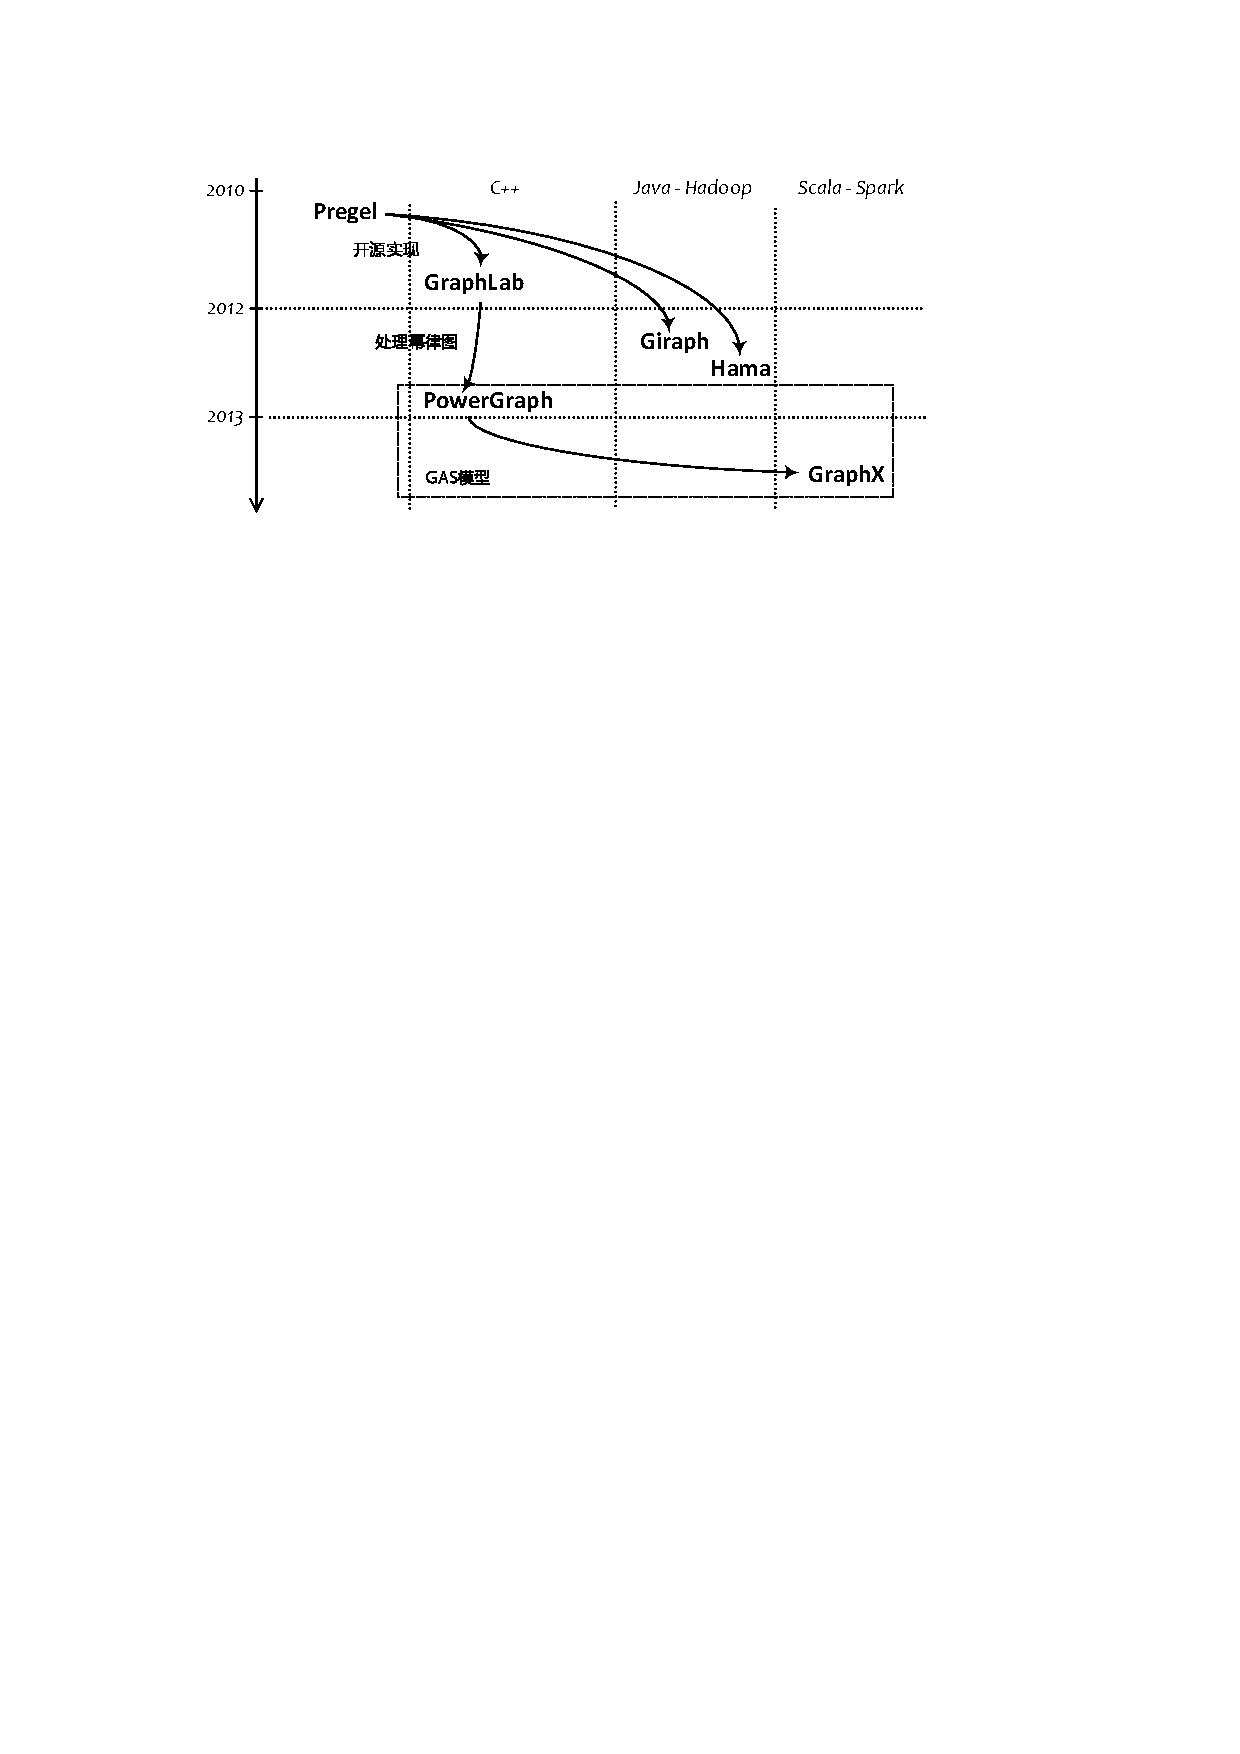
\includegraphics[width=0.80\textwidth]{vis-3-bsp}
        \bicaption{(分布式)图计算框架的发展历程。}{Development of (distributed) graph computing framework.}
        \label{fig:vis-3-bsp}
    \end{figure}

    \begin{enumerate}

        \item ... deleted ...
        \item ... deleted ...
        \item ... deleted ...
            \begin{itemize}
            \item ... deleted ...
            \item ... deleted ...
            \item ... deleted ...
            \end{itemize}

        \item ... deleted ...

            \begin{figure}[!htbp]
                \centering
                %trim option's parameter order: left bottom right top
                % \includegraphics[trim = 30mm 0mm 30mm 0mm, clip, width=0.40\textwidth]{shock_cyn}
                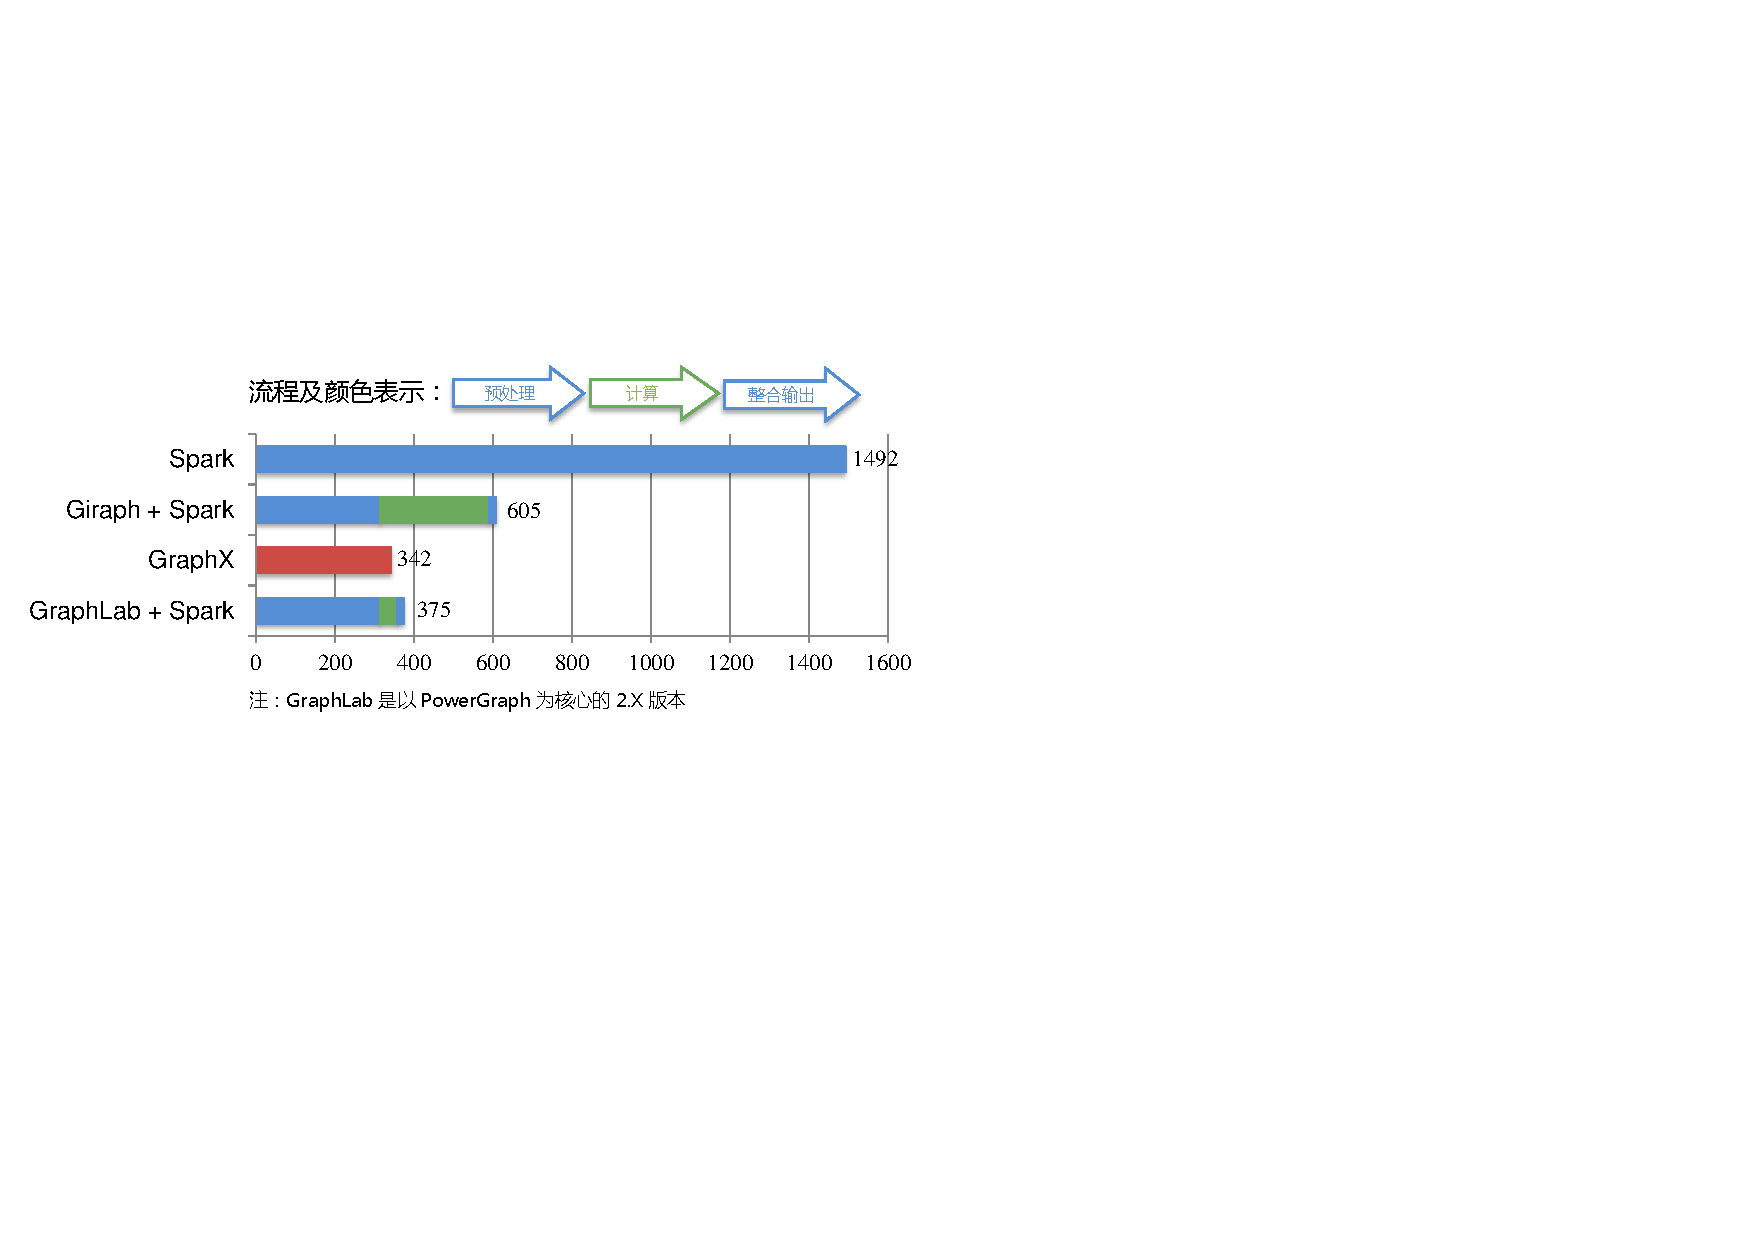
\includegraphics[width=0.85\textwidth]{vis-3-graphxplus}
                \bicaption{Pipeline模式下的性能分析-10次PageRank的运行时间。}{Performance test based on pipeline mode - Times of 10 PageRank iterations.}
                \label{fig:vis-3-graphxplus}
            \end{figure}

 
    \end{enumerate}

    \subsection{大规模图布局算法}

    ... deleted ...
 
    \section{图数据抽样算法}\label{图数据抽样算法}

    ... deleted ...





\section{本章小结}

... deleted ...
\chapter{面向大图的分层抽样算法}\label{chap:面向大图的分层抽样算法}

    \begin{algorithm}[!htbp]
        \small
        \caption{KSS 获取抽样结构$G_s$}\label{alg:k-ss-03}
        \begin{algorithmic}[1]
            \State \textbf{输入:} $V_{sup}$,$C_k$,$S_0,...,S_k$($X_1,...,X_M$),$T$,$p$
            \State \textbf{输出:} $G_s=(V_s,E_s)$
            \State \textbf{foreach} $v \in S_k$ \textbf{do}
            \State     \qquad \textbf{if} $\verb"Corevalues"(\verb"Neighbors"(v))==k$ \textbf{then} $V_{conn} \leftarrow v$
            \State     \qquad \textbf{else} $V_{disconn} \leftarrow v$
            \State \textbf{end }
            \State $i \leftarrow k-T$
            \State \textbf{while} $i > 0$ \textbf{do}
            \State     \qquad \textbf{foreach} $v \in S_i$ \textbf{do}
            \State     \qquad \qquad \textbf{if} $\verb"Shellvalues"(\verb"Neighbors"(v))\in[i-T,i]$ \textbf{then} $V_{conn} \leftarrow v$
            \State     \qquad \qquad  \textbf{else} $V_{disconn} \leftarrow v$
            \State     \qquad \textbf{end }
            \State     \qquad $V_s+=\verb"Sampling"(V_{conn},~k*p)$
            \State     \qquad $V_s+=\verb"Sampling"(V_{disconn},~(1-k)*p)$
            \State     \qquad $i \leftarrow i - T$
            \State \textbf{end while}
            \State $E_s \leftarrow \verb"getEdges"(V_s)$
            \State \textbf{return} $G_s=(V_s,E_s)$
        \end{algorithmic}
    \end{algorithm}


    \begin{figure}[!htbp]
        \begin{subfigure}[b]{0.31\textwidth}
          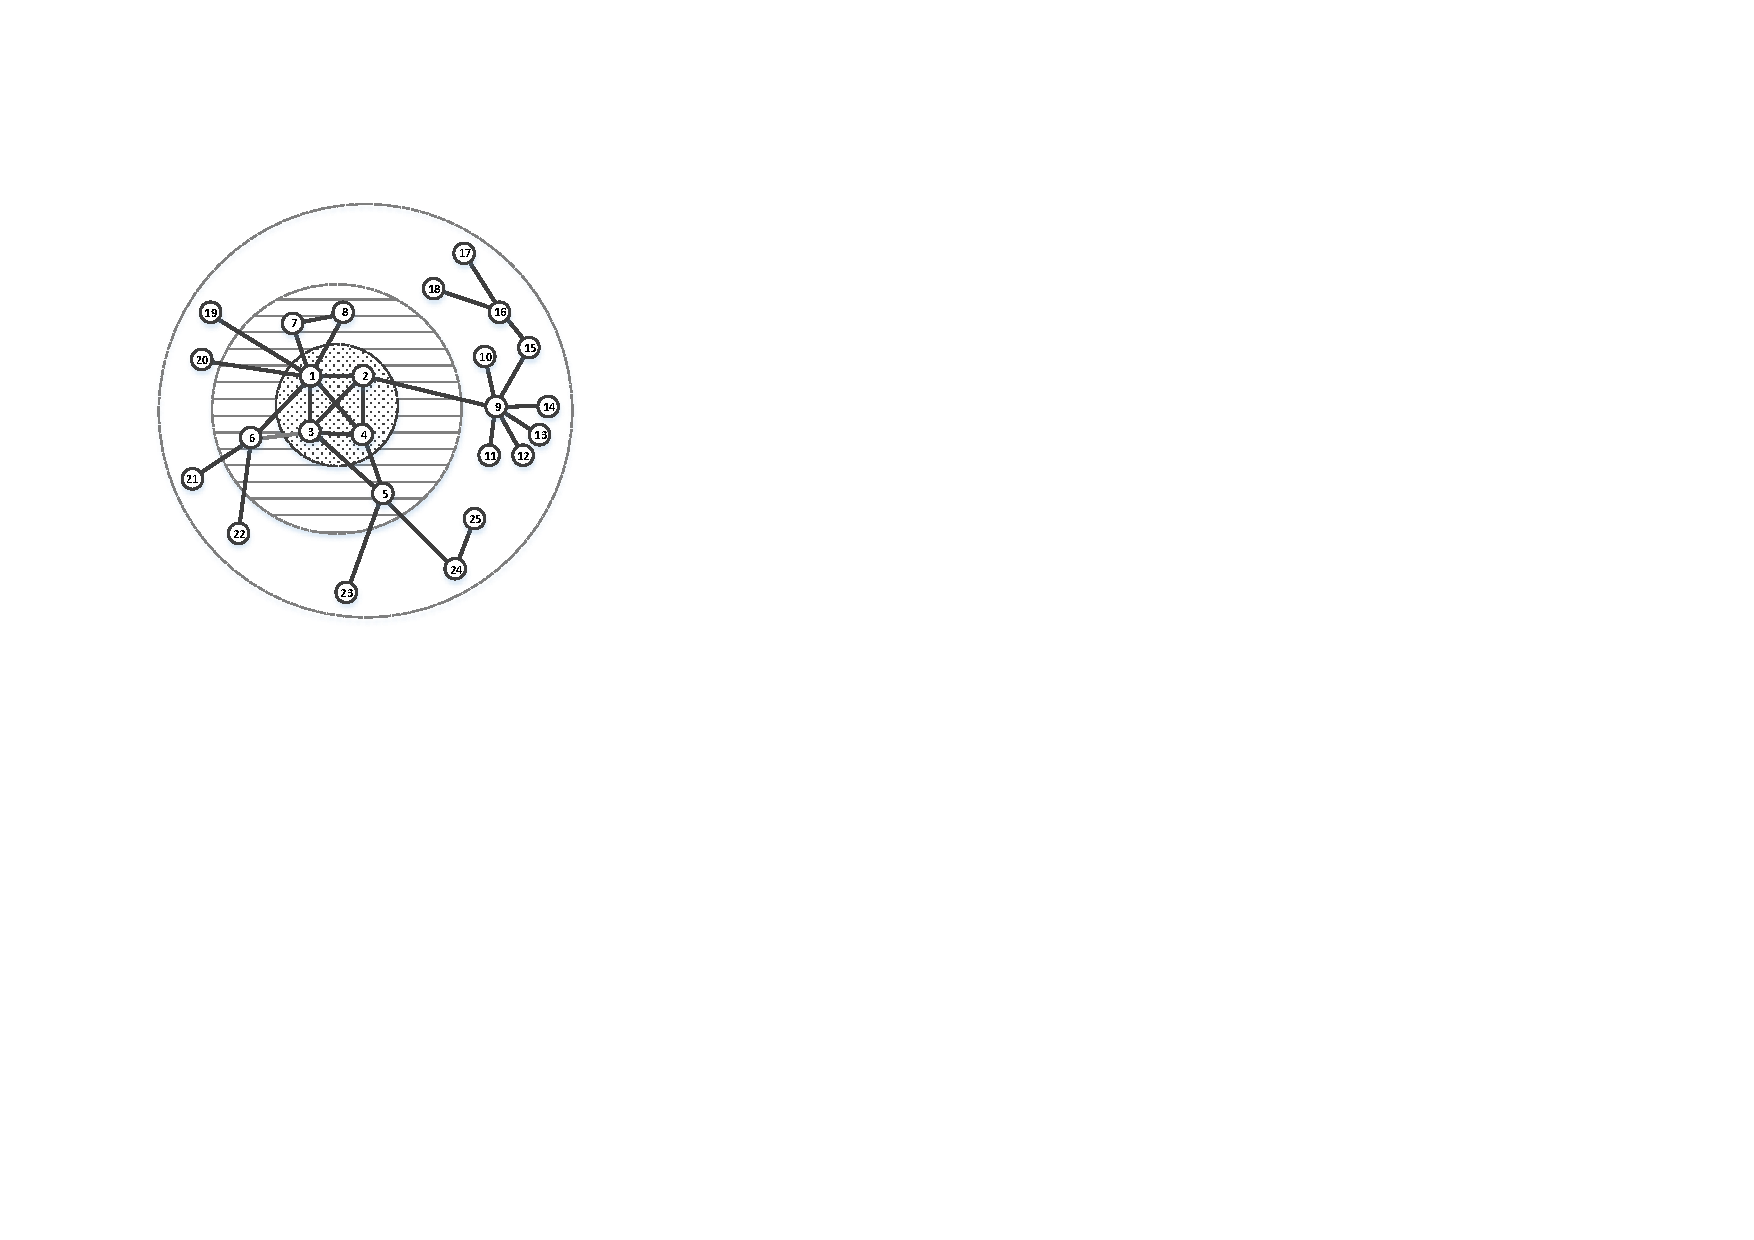
\includegraphics[width=\textwidth]{vis-4-study-a}
          \caption{}
          \label{fig:vis-4-study-a}
        \end{subfigure}
        ~
        \centering
        \begin{subfigure}[b]{0.31\textwidth}
          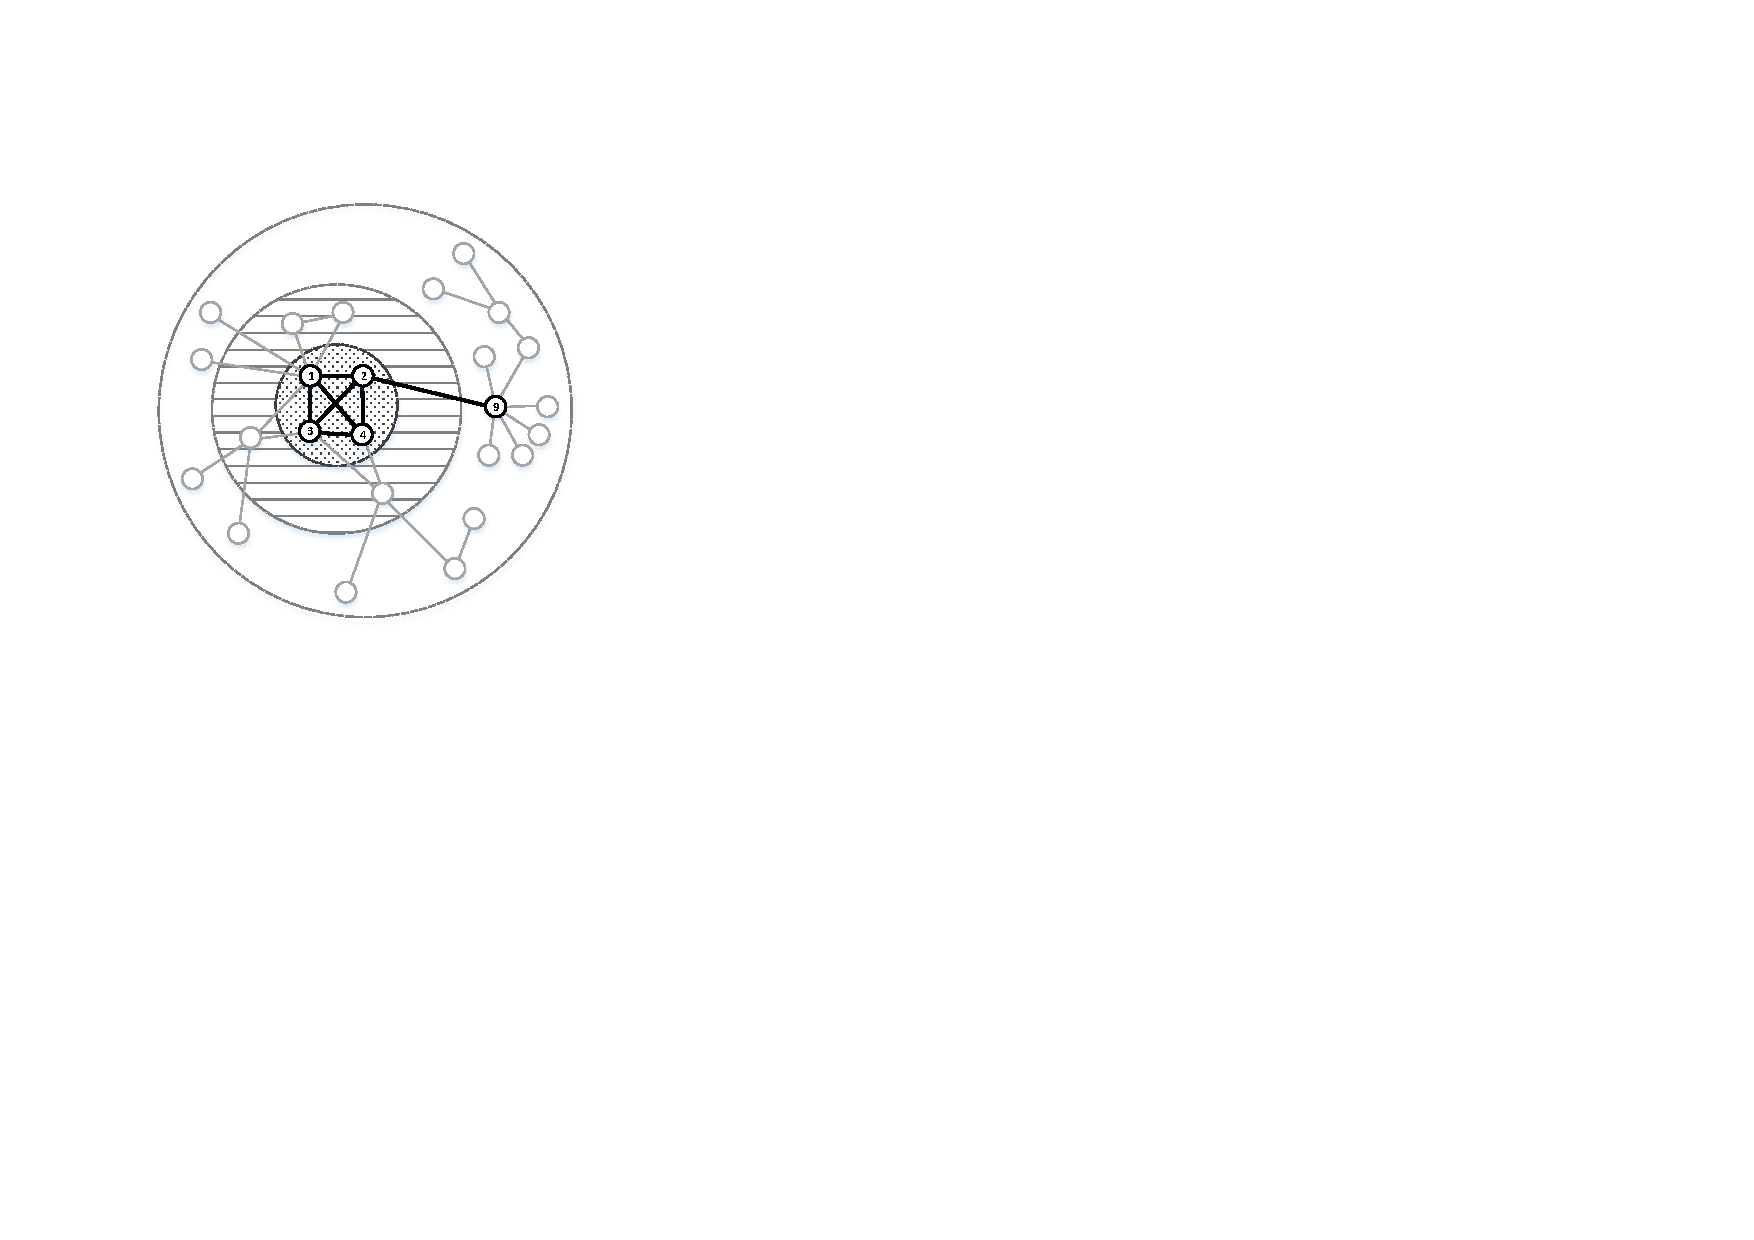
\includegraphics[width=\textwidth]{vis-4-study-b}
          \caption{}
          \label{fig:vis-4-study-b}
        \end{subfigure}%
        ~~%add desired spacing
        \centering
        \begin{subfigure}[b]{0.31\textwidth}
          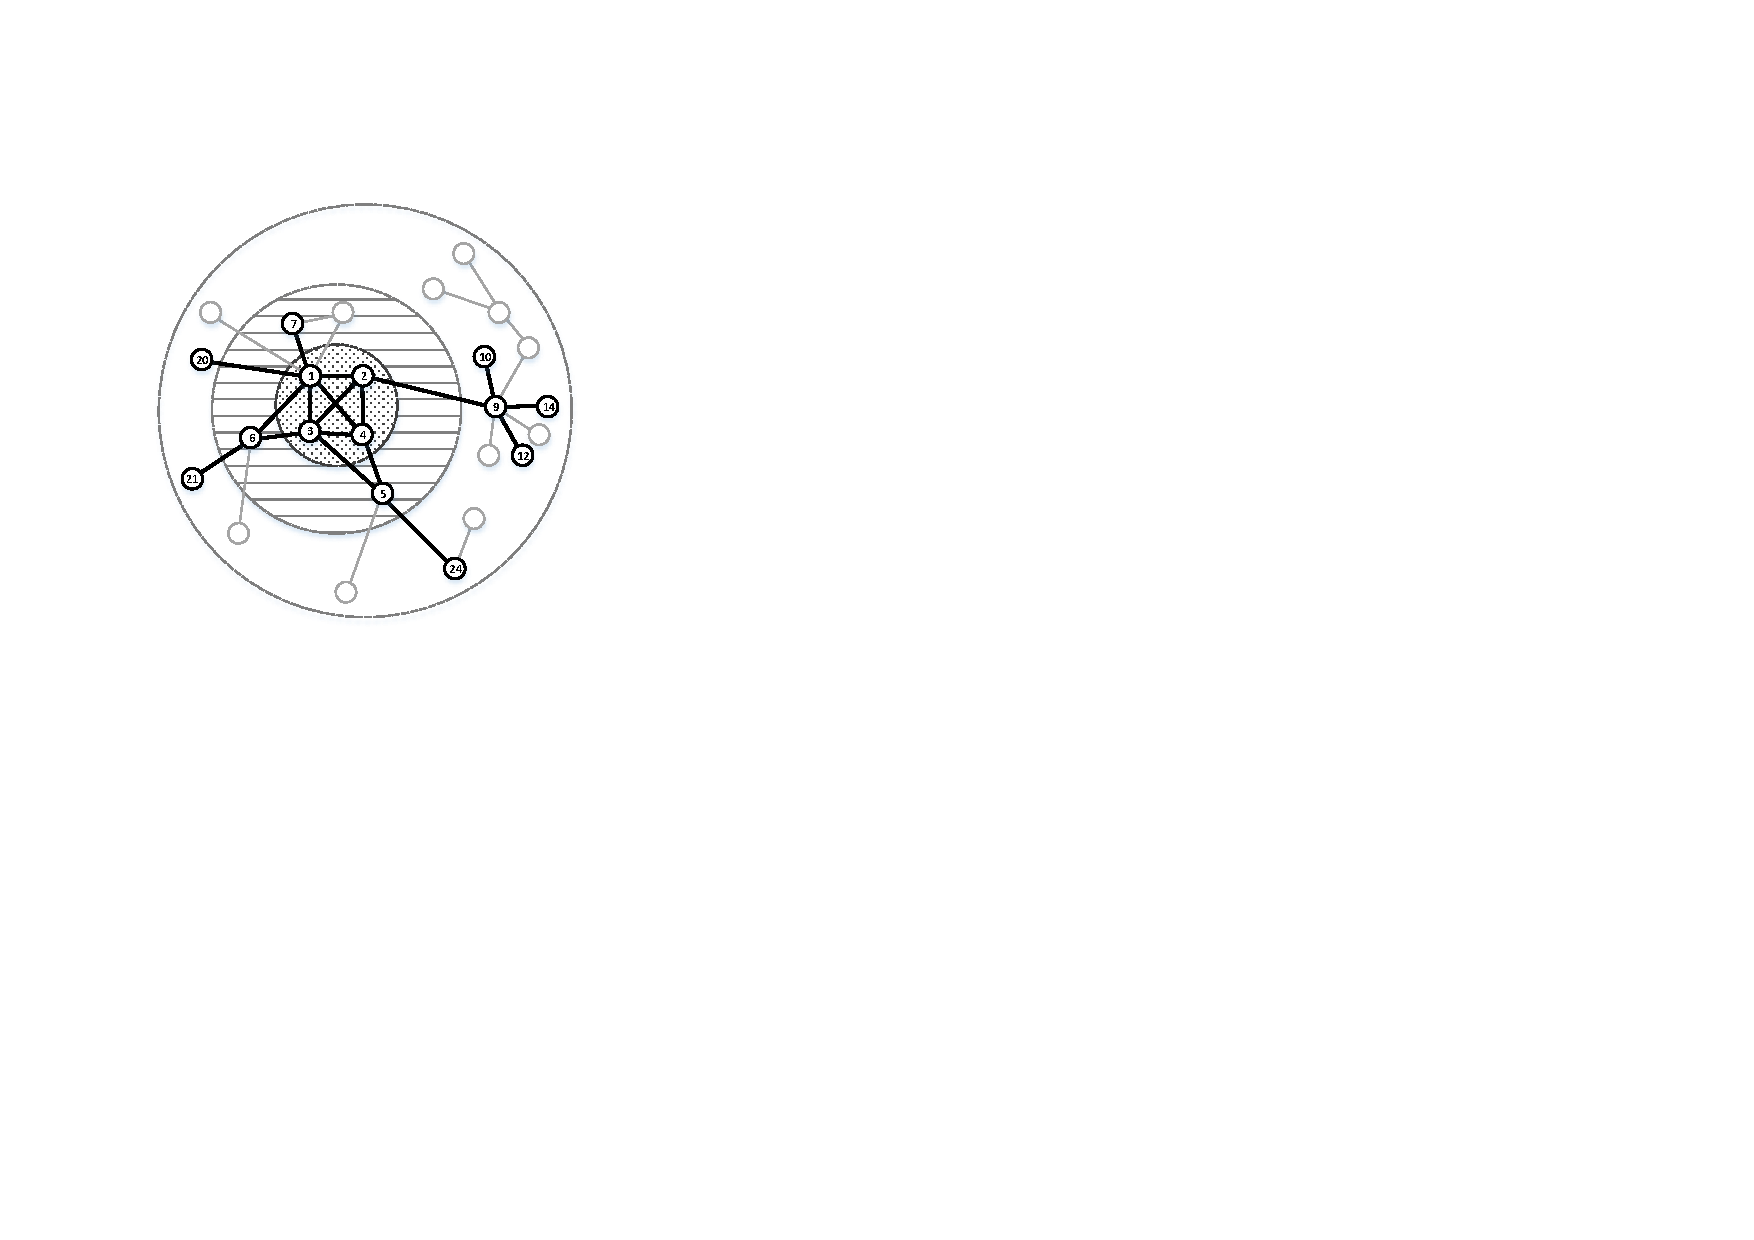
\includegraphics[width=\textwidth]{vis-4-study-c}
          \caption{}
          \label{fig:vis-4-study-c}
        \end{subfigure}%
        \bicaption{KSS抽样示例。(a) 示例结构,(b) 首层结构,(c) 最终结构。 }{Demo case of KSS. (a) Demo graph, (b) First layer structrue, (c) Final layer structure.}
        \label{fig:vis-4-study}
    \end{figure}


    \begin{table}[!htbp]
      \centering
      \bicaption{loc-Gowalla数据集的抽样效果。}{Sampling result of loc-Gowalla data set.}
      \fontsize{10}{10}\selectfont
      \setlength{\tabcolsep}{3mm}{
        \begin{tabular}{clllllll}
        \toprule
        \multicolumn{1}{l}{$Rate(\%)$} & $Algorithm$ & \multicolumn{1}{l}{$SM_d$} & \multicolumn{1}{l}{$V_{gc}^{'}$} & \multicolumn{1}{l}{$V_{cc}^{'}$} & \multicolumn{1}{l}{$V_{av}^{'}$} \\
        \midrule
        \multirow{5}[1]{*}{20} & RN    & 452.898 & 12.408 & 0.501 & 0.192 \\
              & RE    & 206.66 & 2.244 & 0.671 & 0.193 \\
              & SBS   & 239.564 & 1.035 & 0.59  & 1.398 \\
              & SS    & 237.636 & 0.712 & 0.113 & 2.756 \\
              & KSS   & 232.134 & 1.542 & 0.108 & 2.851 \\
        \midrule
        \multirow{5}[2]{*}{40} & RN    & 281.304 & 2.88  & 0.66  & 0.386 \\
              & RE    & 84.086 & 1.114 & 0.684 & 0.387 \\
              & SBS   & 207.437 & 0.869 & 0.567 & 1.446 \\
              & SS    & 167.298 & 0.612 & 0.175 & 2.017 \\
              & KSS   & 133.185 & 1.26  & 0.203 & 1.872 \\
        \midrule
        \multirow{5}[2]{*}{60} & RN    & 105.168 & 1.227 & 0.683 & 0.582 \\
              & RE    & 40.49 & 0.738 & 0.66  & 0.58 \\
              & SBS   & 180.316 & 0.807 & 0.574 & 1.423 \\
              & SS    & 166.767 & 0.516 & 0.295 & 1.451 \\
              & KSS   & 111.889 & 1.043 & 0.407 & 1.299 \\
        \bottomrule
        \end{tabular}%
        }
      \label{tab:3-testa-3}%
    \end{table}%





\chapter{分布式图布局算法}\label{chap:基于KSS抽样的分布式图布局算法}































\chapter{大图可视化原型系统}\label{chap:大图可视交互原型系统}

 
\chapter{总结与展望}\label{chap:总结与展望}

 
%%\chapter{绪论}\label{chap:introduction}

\section{背景}

考虑到许多同学可能缺乏\LaTeX{}使用经验,neuthesis将\LaTeX{}的复杂性高度封装,开放出简单的接口,以便轻易使用。同时,对用\LaTeX{}撰写论文的一些主要难题,如制图、制表、文献索引等,进行了详细说明,并提供了相应的代码样本,理解了上述问题后,对于初学者而言,使用此模板撰写学位论文将不存在实质性的困难。所以,如果你是初学者,请不要直接放弃,因为同样为初学者的我,十分明白让\LaTeX{}简单易用的重要性,而这正是neuthesis所追求和体现的。

该模板基于中国科学院大学学位论文模板causthesis模板发展而来。neuthesis模板满足最新的东北大学博士学位论文排版要求和封面打印设定。兼顾操作系统:Windows,Linux,MacOS 和\LaTeX{}编译引擎:pdflatex,xelatex,lualatex。支持中文书签、中文渲染、中文粗体显示、拷贝PDF中的文本到其他文本编辑器等特性。此外,对模板的文档结构进行了精心设计,撰写了编译脚本提高模板的易用性和使用效率。

neuthesis的目标在于简化学位论文的撰写,利用\LaTeX{}格式与内容分离的特征,模板将格式设计好后,作者可只需关注论文内容。 同时,neuthesis有着整洁一致的代码结构和扼要的注解,对文档的仔细阅读可为初学者提供一个学习\LaTeX{}的窗口。

\section{系统要求}\label{sec:system}

\href{https://github.com/mervin0502/neuthesis}{\texttt{neuthesis}} 宏包可以在目前主流的 \href{https://en.wikibooks.org/wiki/LaTeX/Introduction}{\LaTeX{}} 编译系统中使用,例如C\TeX{}套装 (请勿混淆C\TeX{}套装与ctex宏包。C\TeX{}套装是集成了许多\LaTeX{}组件的\LaTeX{}编译系统,因已停止维护,\textbf{不再建议使用}。 \href{https://ctan.org/pkg/ctex?lang=en}{ctex} 宏包如同neuthesis,是\LaTeX{}命令集,其维护状态活跃,并被主流的\LaTeX{}编译系统默认集成,是几乎所有\LaTeX{}中文文档的核心架构。)、MiK\TeX{}(维护较不稳定,\textbf{不太推荐使用})、\TeX{}Live。推荐的 \href{https://en.wikibooks.org/wiki/LaTeX/Installation}{\LaTeX{}编译系统} 和 \href{https://en.wikibooks.org/wiki/LaTeX/Installation}{\LaTeX{}文本编辑器} 为

\LaTeX{}编译系统 (如\TeX{}Live) 用于提供编译环境,\LaTeX{}文本编辑器 (如Texmaker) 用于编辑\TeX{}源文件。请从各软件的官网下载安装程序,勿使用其它程序源。\textbf{\LaTeX{}编译系统和\LaTeX{}编辑器分别安装成功后,用户即完成了\LaTeX{}的系统配置},无需其他手动干预和配置。若用户的系统原带有旧版的\LaTeX{}编译系统并想安装新版,请\textbf{先卸载干净旧版再安装新版}。

\section{问题反馈}

关于\LaTeX{}的知识性问题,请查阅 
\href{https://github.com/mohuangrui/ucasthesis/wiki}{\LaTeX{}知识小站} 和 
\href{https://en.wikibooks.org/wiki/LaTeX}{\LaTeX{} Wikibook}。

关于模板编译和样式设计的问题,请\textbf{先仔细阅读此说明文档,特别是“常见问题”(章节~\ref{sec:qa})}。若问题仍无法得到解决,请\textbf{先将问题理解清楚并描述清楚,再将问题反馈}至 \href{https://github.com/mervin0502/neuthesis/issues}{Github/neuthesis/issues}。

欢迎大家有效地反馈模板不足之处,一起不断改进模板。希望大家向同事积极推广\LaTeX{},一起更高效地做科研。

\section{模板下载}

\begin{center}
    \href{https://github.com/mervin0502/neuthesis}{Github/neuthesis}: \url{https://github.com/mervin0502/neuthesis}
\end{center}


%%\chapter{LaTeX使用说明}\label{chap:guide}

为方便使用及更好地展示LaTeX排版的优秀特性,neuthesis的框架和文件体系进行了细致地处理,尽可能地对各个功能和板块进行了模块化和封装,对于初学者来说,众多的文件目录也许一开始让人觉得有些无所适从,但阅读完下面的使用说明后,会发现原来使用思路是简单而清晰的,而且,当对LaTeX有一定的认识和了解后,会发现其相对Word类排版系统极具吸引力的优秀特性。所以,如果是初学者,请不要退缩,请稍加尝试和坚持,以领略到LaTeX的非凡魅力,并可以通过阅读相关资料如LaTeX Wikibook\cite{wikibook2014latex}来完善自己的使用知识。

\section{先试试效果}

\begin{enumerate}
    \item 安装软件:根据所用操作系统和章节~`\ref{sec:system}`中的信息安装LaTeX编译环境。
    \item 获取模板:下载 \href{https://github.com/mervin0502/neuthesis}{neuthesis} 模板并解压。neuthesis模板不仅提供了相应的类文件,同时也提供了包括参考文献等在内的完成学位论文的一切要素,所以,下载时,推荐下载整个neuthesis文件夹,而不是单独的文档类。
    \item 编译模板:
        \begin{enumerate}
            \item Windows:双击运行artratex.bat脚本。
            \item Linux或MacOS: {\scriptsize \verb|terminal| -> \verb|chmod +x ./artratex.sh| -> \verb|./artratex.sh xa|}
            \item 任意系统:都可使用LaTeX编辑器打开Thesis.tex文件并选择xelatex编译引擎进行编译。
        \end{enumerate}
    \item 错误处理:若编译中遇到了问题,请先查看“常见问题”(章节~\ref{sec:qa})。
\end{enumerate}

编译完成即可获得本PDF说明文档。而这也完成了学习使用neuthesis撰写论文的一半进程。什么?这就学成一半了,这么简单???,是的,就这么简单!

\section{文档目录简介}

\subsection{Thesis.tex}

Thesis.tex为主文档,其设计和规划了论文的整体框架,通过对其的阅读可以了解整个论文框架的搭建。

\subsection{编译脚本}

\begin{itemize}
    \item Windows:双击Dos脚本artratex.bat可得全编译后的PDF文档,其存在是为了帮助不了解LaTeX编译过程的初学者跨过编译这第一道坎,请勿通过邮件传播和接收此脚本,以防范Dos脚本的潜在风险。
    \item Linux或MacOS:在terminal中运行
        \begin{itemize}
            \item \verb|./artratex.sh xa|:获得全编译后的PDF文档
            \item \verb|./artratex.sh x|:快速编译模式
        \end{itemize}
    \item 全编译指运行 \verb|xelatex+bibtex+xelatex+xelatex| 以正确生成所有的引用链接,如目录,参考文献及引用等。在写作过程中若无添加新的引用,则可用快速编译,即只运行一遍LaTeX编译引擎以减少编译时间。
\end{itemize}

\subsection{Tmp文件夹}

运行编译脚本后,编译所生成的文档皆存于Tmp文件夹内,包括编译得到的PDF文档,其存在是为了保持工作空间的整洁,因为好的心情是很重要的。

\subsection{Style文件夹}

包含neuthesis文档类的定义文件和配置文件,通过对它们的修改可以实现特定的模版设定。若需更新模板,一般只需用新的样式文件替换旧的即可。

\begin{enumerate}
    \item neuthesis.cls:文档类定义文件,论文的最核心的格式即通过它来定义的。
    \item neuthesis.cfg:文档类配置文件,设定如目录显示为“目~录”而非“目录”。
    \item artratex.sty: 常用宏包及文档设定,如参考文献样式、文献引用样式、页眉页脚设定等。这些功能具有开关选项,常只需在Thesis.tex中的如下命令中进行启用即可,一般无需修改artratex.sty本身。
        
        \path{\usepackage[options]{artratex}} 
    \item artracom.sty:自定义命令以及添加宏包的推荐放置位置。
\end{enumerate}

\subsection{Tex文件夹}

文件夹内为论文的所有实体内容,正常情况下,这也是\textbf{使用neuthesis撰写学文论文时,主要关注和修改的一个位置,注:所有文件都必须采用UTF-8编码,否则编译后将出现乱码文本},详细分类介绍如下:

\begin{itemize}
    \item Frontpage.tex:为论文中英文封面及中英文摘要。\textbf{论文封面会根据英文学位名称如Bachelor,Master,或是Doctor自动切换为相应的格式}。
    \item Mainmatter.tex:索引需要出现的Chapter。开始写论文时,可以只索引当前章节,以快速编译查看,当论文完成后,再对所有章节进行索引即可。
    \item Chap{\_}xxx.tex:为论文主体的各个章节,可根据需要添加和撰写。
    \item Appendix.tex:为附录内容
    \item Backmatter.tex:为发表文章信息和致谢部分等。
\end{itemize}

\subsection{Img文件夹}

用于放置论文中所需要的图类文件,支持格式有:.jpg, .png, .pdf。其中,\verb|neu_logo.pdf|为东北大学校徽。不建议为各章节图片建子目录,即使图片众多,若命名规则合理,图片查询亦是十分方便。

\subsection{Biblio文件夹}

\begin{enumerate}
    \item ref.bib:参考文献信息库。
    \item gbt7714-xxx.bst:符合国标的文献样式定义文件。由 \href{https://github.com/zepinglee/gbt7714-bibtex-style}{zepinglee}  开发,并满足最新国标要求。与文献样式有关的问题,请查阅开发者所提供的文档,并建议适当追踪其更新。
\end{enumerate}

\section{常见使用问题}\label{sec:qa}

\begin{enumerate}
    \item 模板每次发布前,都已在Windows,Linux,MacOS系统上测试通过。下载模板后,若编译出现错误,则请见 \href{https://github.com/mervin0502/neuthesis/wiki}{neuthesis和LaTeX知识小站} 的 \href{https://github.com/mervin0502/neuthesis/wiki/%E7%BC%96%E8%AF%91%E6%8C%87%E5%8D%97}{编译指南}。

    \item 模板文档的编码为UTF-8编码。所有文件都必须采用UTF-8编码,否则编译后生成的文档将出现乱码文本。若出现文本编辑器无法打开文档或打开文档乱码的问题,请检查编辑器对UTF-8编码的支持。如果使用WinEdt作为文本编辑器(\textbf{不推荐使用}),应在其Options -> Preferences -> wrapping选项卡下将两种Wrapping Modes中的内容:
        
        TeX;HTML;ANSI;ASCII|DTX...
        
        修改为:TeX;\textbf{UTF-8|ACP;}HTML;ANSI;ASCII|DTX...
        
        同时,取消Options -> Preferences -> Unicode中的Enable ANSI Format。

    \item 推荐选择xelatex或lualatex编译引擎编译中文文档。编译脚本的默认设定为xelatex编译引擎。你也可以选择不使用脚本编译,如直接使用 LaTeX文本编辑器编译。注:LaTeX文本编辑器编译的默认设定为pdflatex编译引擎,若选择xelatex或lualatex编译引擎,请进入下拉菜单选择。为正确生成引用链接,需要进行全编译。

    \item Texmaker使用简介
        \begin{enumerate}
            \footnotesize
            \item 使用 Texmaker “打开 (Open)” Thesis.tex。
            \item 菜单 “选项 (Options)” -> “设置当前文档为主文档 (Define as Master Document)”
            \item 菜单 “自定义 (User)” -> “自定义命令 (User Commands)” -> “编辑自定义命令 (Edit User Commands)” -> 左侧选择 “command 1”,右侧 “菜单项 (Menu Item)” 填入 Auto Build -> 点击下方“向导 (Wizard)” -> “添加 (Add)”: xelatex + bibtex + xelatex + xelatex + pdf viewer -> 点击“完成 (OK)”
            \item 使用 Auto Build 编译带有未生成引用链接的源文件,可以仅使用 xelatex 编译带有已经正确生成引用链接的源文件。
            \item 编译完成,“查看(View)” PDF,在PDF中 “ctrl+click” 可链接到相对应的源文件。
        \end{enumerate}
    
    \item 模版的设计可能地考虑了适应性。致谢等所有条目都是通过最为通用的

        \verb+\chapter{item name}+  and \verb+\section*{item name}+

        来显式实现的 (请观察Backmatter.tex),从而可以随意添加,放置,和修改,如同一般章节。对于图表目录名称则可在neuthesis.cfg中进行修改。

    \item 设置文档样式: 在artratex.sty中搜索关键字定位相应命令,然后修改
        \begin{enumerate}
            \item 正文行距:启用和设置 \verb|\linespread{1.5}|,默认1.5倍行距。
            \item 参考文献行距:修改 \verb|\setlength{\bibsep}{0.0ex}|
            \item 目录显示级数:修改 \verb|\setcounter{tocdepth}{2}|
            \item 文档超链接的颜色及其显示:修改 \verb|\hypersetup|
        \end{enumerate}

    \item 文档内字体切换方法:
        \begin{itemize}
            \item 宋体:东北大学论文模板neuthesis 或 \textrm{东北大学论文模板neuthesis}
            \item 粗宋体:{\bfseries 东北大学论文模板neuthesis} 或 \textbf{东北大学论文模板neuthesis}
            \item 黑体:{\sffamily 东北大学论文模板neuthesis} 或 \textsf{东北大学论文模板neuthesis}
            \item 粗黑体:{\bfseries\sffamily 东北大学论文模板neuthesis} 或 \textsf{\bfseries 东北大学论文模板neuthesis}
            \item 仿宋:{\ttfamily 东北大学论文模板neuthesis} 或 \texttt{东北大学论文模板neuthesis}
            \item 粗仿宋:{\bfseries\ttfamily 东北大学论文模板neuthesis} 或 \texttt{\bfseries 东北大学论文模板neuthesis}
            \item 楷体:{\itshape 东北大学论文模板neuthesis} 或 \textit{东北大学论文模板neuthesis}
            \item 粗楷体:{\bfseries\itshape 东北大学论文模板neuthesis} 或 \textit{\bfseries 东北大学论文模板neuthesis}
        \end{itemize}

    \item 封面下划线上的文本不居中下划线,这是因为下划线前面还有字头,导致文本只能在页面居中和在下划线上居中二选一。当前封面采取页面居中。如需要调整文本在下划线上的位置,可用 \verb|\hspace{+/- n.0em}| 命令来插入或删除 n 个空格,进行手动调整,比如

        \verb|\advisor{\hspace{+3.0em} xxx~研究员~xxx单位}|
                
    有时下划线看上去粗细不一致,这是显示的问题,打印正常。
\end{enumerate}



%%\chapter{排版格式}\label{chap:format}

\section{引言}
依据中华人民共和国《科学技术报告、学位论文和学术论文的编写格式》和东北大学学位论文格式改编,专为我校申请硕士、博士学位人员撰写打印论文时使用。本格式自发布日起实行。
\section{学位论文主要部分}
学位论文主要部分由前头部分、主体部分和结尾部分组成。
\subsection{前头部分}
\begin{itemize}
    \item 封面
    \item 扉页——题名页(中、英两种)
    \item 声明(独创性声明)
    \item 摘要(中、英两种文字)
    \item 目录
    \item 插图和附表清单(只限必要时)
    \item 缩略字、缩写词、符号、单位表(只限必要时)
    \item 名词术语注释表(只限必要时)
\end{itemize}

\subsection{主体部分}
\begin{itemize}
    \item 绪论(前言、引言、绪言)
    \item 正文
    \item 讨论、结论和建议
\end{itemize}
\subsection{结尾部分(只限必要时采用)}
\begin{itemize}
    \item 参考文献
    \item 致谢
    \item 攻读博士学位期间取得的学术成果
    \item 作者从事科学研究和学习经历的简历
    \item 可供参考的文献题录(只限必要时采用)
    \item 索引(只限必要时采用)
\end{itemize}

\section{版式}
纸张大小:纸的尺寸为标准A4复印纸(210mm×297mm)。

版芯(打印尺寸):160mm×247mm(不包括页眉行、页码行)。

正文字体字号:小4号宋体,全文统一。

每页30~35行,每行35~38字。

装订:双面打印印刷,沿长边装订。

页码:页码用阿拉伯数字连续编页,字号与正文字体相同,页底居中,数字两侧用圆点或一字横线修饰,如·3·或-3-。

页眉:自摘要页起加页眉,眉体可用单线或双线(二等线、文武线),页眉说明5号楷体,左端“东北大学硕士、博士学位论文”,右端“章号章题”。

封面:东北大学研究生(博士或硕士)学位论文标准封面(双A4)。

\section{体例}

\subsection{标题}

论文正文按章、条、款、项分级,在不同级的章、条、款、项阿拉伯数字编号之间用点“.”(半角实心下圆点)相隔,最末级编号之后不加点。排版格式见表4.1。

此分级编号法只分至第四级。再分可用(1)、(2)……;(a)、(b)……等。

\begin{table}[htpb]
    \begin{center}
        \bicaption{标题排版格式}{Typesetting format of the heading}
        \begin{tabular}{|l | l | l | l |}
            \hline
            标题       & 字号字体   & 格式        & 举例           \\
            \hline
            第一级(章) & 二号黑体   & 居中,占3行 & 第1章 XXX      \\
            \hline
            第二级(条) & 三号黑体   & 居左,占2行 & 1.1 XXXXXX     \\
            \hline
            第三级(款) & 四号黑体   & 居左,占2行 & 1.1.1 XXXXXX   \\
            \hline
            第四级(项) & 小四号黑体 & 居左,占1行 & 1.1.1.1 XXXXXX \\
            \hline
        \end{tabular}
    \end{center}
\end{table}

摘要、目录、参考文献、致谢、攻读博士学位期间取得的学术成果、个人简历等标题作为第一级标题排版。

\subsection{正文}
汉字字体字号:正文字体小4号宋体。

外文、数字字号与同行汉字字号相同,字体用WORD系统中的Time New Roman体或相近字体。

\subsubsection{插图}
插图包括图解、示意图、构造图、曲线图、框图、流程图、布置图、地图、照片、图版等。插图注明项有图号、图题、图例。图号编码用章序号。如“图2.1“表示第2章第1图。图号与图题文字间置一字空格,置于图的正下方,图题用5号字,字体可用宋体,须全文统一。图中标注符号文字字号不大于图题的字号。

论文中图片的插入通常分为单图和多图,下面分别加以介绍:

单图插入:假设插入名为\verb|tc_q_criteria|(后缀可以为.jpg、.png、.pdf,下同)的图片,其效果如图\ref{fig:tc_q_criteria}。
\begin{figure}[!htbp]
    \centering
    \includegraphics[width=0.40\textwidth]{tc_q_criteria}
    \bicaption{Q判据等值面图,同时测试一下一个很长的标题,比如这真的是一个很长很长很长很长很长很长很长很长的标题。}{Isocontour of Q criteria, at the same time, this is to test a long title, for instance, this is a really very long very long very long very long very long title.}
    \label{fig:tc_q_criteria}
\end{figure}

如果插图的空白区域过大,以图片\verb|shock_cyn|为例,自动裁剪如图\ref{fig:shock_cyn}。
\begin{figure}[!htbp]
    \centering
    %trim option's parameter order: left bottom right top
    % \includegraphics[trim = 30mm 0mm 30mm 0mm, clip, width=0.40\textwidth]{shock_cyn}
    \includegraphics[width=0.40\textwidth]{shock_cyn}
    \bicaption{激波圆柱作用。}{Shock-cylinder interaction.}
    \label{fig:shock_cyn}
\end{figure}

多图的插入如图\ref{fig:oaspl},多图不应在子图中给文本子标题,只要给序号,并在主标题中进行引用说明。
\begin{figure}[!htbp]
    \centering
    \begin{subfigure}[b]{0.35\textwidth}
      \includegraphics[width=\textwidth]{oaspl_a}
      \caption{}
      \label{fig:oaspl_a}
    \end{subfigure}%
    ~%add desired spacing
    \begin{subfigure}[b]{0.35\textwidth}
      \includegraphics[width=\textwidth]{oaspl_b}
      \caption{}
      \label{fig:oaspl_b}
    \end{subfigure}
    \begin{subfigure}[b]{0.35\textwidth}
      \includegraphics[width=\textwidth]{oaspl_c}
      \caption{}
      \label{fig:oaspl_c}
    \end{subfigure}%
    ~%add desired spacing
    \begin{subfigure}[b]{0.35\textwidth}
      \includegraphics[width=\textwidth]{oaspl_d}
      \caption{}
      \label{fig:oaspl_d}
    \end{subfigure}
    \bicaption{总声压级。(a) 这是子图说明信息,(b) 这是子图说明信息,(c) 这是子图说明信息,(d) 这是子图说明信息。}{OASPL.(a) This is the explanation of subfig, (b) This is the explanation of subfig, (c) This is the explanation of subfig, (d) This is the explanation of subfig.}
    \label{fig:oaspl}
\end{figure}

\subsubsection{表}
表的一般格式是数据依序竖排,内容和项目由左至右横读,通版排版。表号也用章序号编码,如:表2.1是第2章中的第1表。表应有表题,与表号之间空1~2字,置于表的上方居中,用5号宋体,须全文统一。表中的内容和项目字号不大于图题的字号。

请见表~\ref{tab:sample}。制表的更多范例,请见 \href{https://en.wikibooks.org/wiki/LaTeX/Tables}{WiKibook Tables}。
\begin{table}[!htbp]
    \bicaption{这是一个样表。}{This is a sample table.}
    \label{tab:sample}
    \centering
    \footnotesize% fontsize
    \setlength{\tabcolsep}{4pt}% column separation
    \renewcommand{\arraystretch}{1.2}%row space 
    \begin{tabular}{lcccccccc}
        \hline
        Row number & \multicolumn{8}{c}{This is a multicolumn} \\
        %\cline{2-9}% partial hline from column i to column j
        \hline
        Row 1 & $1$ & $2$ & $4$ & $5$ & $6$ & $7$ & $8$\\
        Row 2 & $1$ & $2$ & $4$ & $5$ & $6$ & $7$ & $8$\\
        Row 3 & $1$ & $2$ & $4$ & $5$ & $6$ & $7$ & $8$\\
        Row 4 & $1$ & $2$ & $4$ & $5$ & $6$ & $7$ & $8$\\
        \hline
    \end{tabular}
\end{table}


\subsubsection{公式}
公式包括数学、物理和化学公式。正文中引用的公式、算式或方程式等可以按章序号用阿拉伯数字编号(式号),如:式(2.1)表示第2章第1式,公式一般单行居中排版与上下文分开,式号与公式同行居右排版。

比如Navier-Stokes方程:
\begin{equation} \label{eq:ns}
    \begin{cases}
        \frac{\partial \rho}{\partial t} + \nabla\cdot(\rho\Vector{V}) = 0 \ \mathrm{times\ font\ test}\\
        \frac{\partial (\rho\Vector{V})}{\partial t} + \nabla\cdot(\rho\Vector{V}\Vector{V}) = \nabla\cdot\Tensor{\sigma} \ \text{times font test}\\
        \frac{\partial (\rho E)}{\partial t} + \nabla\cdot(\rho E\Vector{V}) = \nabla\cdot(k\nabla T) + \nabla\cdot(\Tensor{\sigma}\cdot\Vector{V})
    \end{cases}
\end{equation}
\begin{equation}
    \frac{\partial }{\partial t}\int\limits_{\Omega} u \, \mathrm{d}\Omega + \int\limits_{S} \unitVector{n}\cdot(u\Vector{V}) \, \mathrm{d}S = \dot{\phi}
\end{equation}

数学公式常用命令请见 \href{https://en.wikibooks.org/wiki/LaTeX/Mathematics}{WiKibook Mathematics}。artracom.sty中对一些常用数据类型如矢量矩阵等进行了封装,这样的好处是如有一天需要修改矢量的显示形式,只需单独修改artracom.sty中的矢量定义即可实现全文档的修改。

\subsubsection{算法}

如见算法~\ref{alg:euclid},详细使用方法请参见文档 \href{https://ctan.org/pkg/algorithmicx?lang=en}{algorithmicx}。

\begin{algorithm}[!htbp]
    \small
    \caption{Euclid's algorithm}\label{alg:euclid}
    \begin{algorithmic}[1]
        \Procedure{Euclid}{$a,b$}\Comment{The g.c.d. of a and b}
        \State $r\gets a\bmod b$
        \While{$r\not=0$}\Comment{We have the answer if r is 0}
        \State $a\gets b$
        \State $b\gets r$
        \State $r\gets a\bmod b$
        \EndWhile\label{euclidendwhile}
        \State \textbf{return} $b$\Comment{The gcd is b}
        \EndProcedure
    \end{algorithmic}
\end{algorithm}

\subsection{附录}
附录中的图、表、公式、参考文献等另行编排序号,与正文分开,也一律用阿拉伯数字编号,但在数码前冠以附录序码。例如:图A.1,式(B.3)等。
\subsection{计量单位}
学位论文一律采用1984年2月27日国务院发布的《中华人民共和国法定计量单位》,并遵照《中华人民共和国法定计量单位使用方法》执行。论文中命名用各种量、单位和符号,必须遵循国家标准GB3100-82,GB3101-82,GB3102/1-13-82等的规定。

单位名称和符号的书写方式,可以采用国际通用符号,也可以用中文名称,但统一采用一种,不要混用。

\subsection{参考文献}

参考文献引用过程以实例进行介绍,假设需要引用名为"Document Preparation System"的文献,步骤如下:

1)使用Google Scholar搜索Document Preparation System,在目标条目下点击Cite,展开后选择Import into BibTeX打开此文章的BibTeX索引信息,将它们copy添加到ref.bib文件中(此文件位于Biblio文件夹下)。

2)索引第一行 \verb|@article{lamport1986document,|中 \verb|lamport1986document| 即为此文献的label (\textbf{中文文献也必须使用英文label},一般遵照:姓氏拼音+年份+标题第一字拼音的格式),想要在论文中索引此文献,有两种索引类型:

文本类型:\verb|\citet{lamport1986document}|。正如此处所示 \citet{lamport1986document}; 

括号类型:\verb|\citep{lamport1986document}|。正如此处所示 \citep{lamport1986document}。

\textbf{多文献索引用英文逗号隔开}:

\verb|\citep{lamport1986document, chu2004tushu, chen2005zhulu}|。正如此处所示 \citep{lamport1986document,chu2004tushu,chen2005zhulu}

更多例子如:

\citet{walls2013drought}根据...的研究,首次提出...。其中关于...\citep{walls2013drought},是当前中国...得到迅速发展的研究领域\citep{chen1980zhongguo}。引用同一著者在同一年份出版的多篇文献时,在出版年份之后用
英文小写字母区别,如:\citep{yuan2012lana,yuan2012lanb,yuan2012lanc}。同一处引用多篇文献时,按出版年份由近及远依次标注,中间用
分号分开。例如\citep{chen1980zhongguo,stamerjohanns2009mathml,hls2012jinji,niu2013zonghe}。

使用著者-出版年制(authoryear)式参考文献样式时,中文文献必须在BibTeX索引信息的 \textbf{key} 域(请参考ref.bib文件)填写作者姓名的拼音,才能使得文献列表按照拼音排序。参考文献表中的条目(不排序号),先按语种分类排列,语种顺 序是:中文、日文、英文、俄文、其他文种。然后,中文按汉语拼音字母顺序排列,日文按第一著者的姓氏笔画排序,西文和 俄文按第一著者姓氏首字母顺序排列。如中\cite{niu2013zonghe}、日\cite{Bohan1928}、英\cite{stamerjohanns2009mathml}、俄\cite{Dubrovin1906}。

如此,即完成了文献的索引,请查看下本文档的参考文献一章,看看是不是就是这么简单呢?是的,就是这么简单!

不同文献样式和引用样式,如著者-出版年制(authoryear)、顺序编码制(numbers)、上标顺序编码制(super)可在Thesis.tex中对artratex.sty调用实现,如:
\begin{itemize}
    \footnotesize
    \item \verb+\usepackage[numbers]{artratex}+ $\%$ 文本: Jones [1]; 括号: [1]
    \item \verb+\usepackage[super]{artratex}+ $\%$ 文本: Jones 上标[1]; 括号: 上标[1]
    \item \verb+\usepackage[authoryear]{artratex}+ $\%$ 文本: Jones (1995); 括号: (Jones, 1995)
    \item \verb+\usepackage[alpha]{artratex}+ $\%$ 文本: 不可用; 括号: [Jon95]
\end{itemize}

当前文档的默认参考文献样式为\textbf{authoryear}。若在上标(\textbf{super})模式下,希望在特定位置将上标改为嵌入式标,可使用

文本类型:\verb|\citens{lamport1986document,chen2005zhulu}|。

正如此处所示\cite{lamport1986document,chen2005zhulu}

括号类型:\verb|\citens{lamport1986document,chen2005zhulu}|。

正如此处所示\cite{lamport1986document,chen2005zhulu}

参考文献索引更为详细的信息,请见 \href{https://github.com/zepinglee/gbt7714-bibtex-style}{zepinglee} 和 \href{https://en.wikibooks.org/wiki/LaTeX/Bibliography_Management}{WiKibook Bibliography}。


参考文献采用顺序号编号体系。

专著格式: 

[序号] 编著者. 书名[M]. 出版地:出版社,年代,起止页码.

期刊论文格式: 

[序号] 作者. 论文名称[J]. 期刊名称,年度,卷(期):起止页码.

学位论文格式: 

[序号] 作者. 学位论文名称[D]. 发表地:学位授予单位,年度.

参考文献举例: 

[1] 张毅. 铸造工艺CAD及其应用[M]. 北京:机械工业出版社,1994,14-15. 

[2] Huang S C, Huang Y M, Shieh S M. Vibration and stability of a rotating shaft containing a transerse crack [J]. J Sound and Vibration, 1993, 162(3): 387-401.

[3] 周丽. 机械式挖掘机工作装置的优化与仿真[D]. 沈阳:东北大学,2000.


\subsection{攻读博士学位期间取得的学术成果}

期刊格式:
[序号] 作者. 论文名称[J]. 期刊名称,年度,卷(期):起止页码. (检索情况)(对应论文章
节)

专利格式:

[序号] 专利申请者. 专利题名:专利国别,专利号[P]. 发布日期. (对应论文章节)

示例:

[1] Huang S C, Huang Y M, Shieh S M. Vibration and stability of a rotating shaft containing a transerse crack[J]. J Sound and Vibration, 1993, 162(3): 387-401. (SCI检索)(对应论文第四章)

[2] 高航,张立成,周士昌. 高压辊磨机液压系统及其动态特性[J]. 东北大学学报,2000,21(1):38-40. (EI检索)(对应论文第五章)

[3] 刘加林. 多功能一次性压舌板:中国,92214985.2[P]. 1993-04-14. (对应论文第四章)


注:双盲评审版学位论文中须隐去所有作者(申请者)姓名,仅标注排序即可。

示例:

[1] 第一作者. Vibration and stability of a rotating shaft containing a transerse crack[J]. J Sound and Vibration, 1993, 162(3): 387-401. (SCI检索)(对应论文第四章)

[2] 第二作者. 高压辊磨机液压系统及其动态特性[J]. 东北大学学报,2000,21(1):38-40. (EI检索)(对应论文第五章)

[3] 第二排序. 多功能一次性压舌板:中国,92214985.2[P]. 1993-04-14. (对应论文第四章)





% \chapter{LaTeX使用说明}\label{chap:guide}

为方便使用及更好地展示LaTeX排版的优秀特性,neuthesis的框架和文件体系进行了细致地处理,尽可能地对各个功能和板块进行了模块化和封装,对于初学者来说,众多的文件目录也许一开始让人觉得有些无所适从,但阅读完下面的使用说明后,会发现原来使用思路是简单而清晰的,而且,当对LaTeX有一定的认识和了解后,会发现其相对Word类排版系统极具吸引力的优秀特性。所以,如果是初学者,请不要退缩,请稍加尝试和坚持,以领略到LaTeX的非凡魅力,并可以通过阅读相关资料如LaTeX Wikibook\cite{wikibook2014latex}来完善自己的使用知识。

\section{先试试效果}

\begin{enumerate}
    \item 安装软件:根据所用操作系统和章节~`\ref{sec:system}`中的信息安装LaTeX编译环境。
    \item 获取模板:下载 \href{https://github.com/mervin0502/neuthesis}{neuthesis} 模板并解压。neuthesis模板不仅提供了相应的类文件,同时也提供了包括参考文献等在内的完成学位论文的一切要素,所以,下载时,推荐下载整个neuthesis文件夹,而不是单独的文档类。
    \item 编译模板:
        \begin{enumerate}
            \item Windows:双击运行artratex.bat脚本。
            \item Linux或MacOS: {\scriptsize \verb|terminal| -> \verb|chmod +x ./artratex.sh| -> \verb|./artratex.sh xa|}
            \item 任意系统:都可使用LaTeX编辑器打开Thesis.tex文件并选择xelatex编译引擎进行编译。
        \end{enumerate}
    \item 错误处理:若编译中遇到了问题,请先查看“常见问题”(章节~\ref{sec:qa})。
\end{enumerate}

编译完成即可获得本PDF说明文档。而这也完成了学习使用neuthesis撰写论文的一半进程。什么?这就学成一半了,这么简单???,是的,就这么简单!

\section{文档目录简介}

\subsection{Thesis.tex}

Thesis.tex为主文档,其设计和规划了论文的整体框架,通过对其的阅读可以了解整个论文框架的搭建。

\subsection{编译脚本}

\begin{itemize}
    \item Windows:双击Dos脚本artratex.bat可得全编译后的PDF文档,其存在是为了帮助不了解LaTeX编译过程的初学者跨过编译这第一道坎,请勿通过邮件传播和接收此脚本,以防范Dos脚本的潜在风险。
    \item Linux或MacOS:在terminal中运行
        \begin{itemize}
            \item \verb|./artratex.sh xa|:获得全编译后的PDF文档
            \item \verb|./artratex.sh x|:快速编译模式
        \end{itemize}
    \item 全编译指运行 \verb|xelatex+bibtex+xelatex+xelatex| 以正确生成所有的引用链接,如目录,参考文献及引用等。在写作过程中若无添加新的引用,则可用快速编译,即只运行一遍LaTeX编译引擎以减少编译时间。
\end{itemize}

\subsection{Tmp文件夹}

运行编译脚本后,编译所生成的文档皆存于Tmp文件夹内,包括编译得到的PDF文档,其存在是为了保持工作空间的整洁,因为好的心情是很重要的。

\subsection{Style文件夹}

包含neuthesis文档类的定义文件和配置文件,通过对它们的修改可以实现特定的模版设定。若需更新模板,一般只需用新的样式文件替换旧的即可。

\begin{enumerate}
    \item neuthesis.cls:文档类定义文件,论文的最核心的格式即通过它来定义的。
    \item neuthesis.cfg:文档类配置文件,设定如目录显示为“目~录”而非“目录”。
    \item artratex.sty: 常用宏包及文档设定,如参考文献样式、文献引用样式、页眉页脚设定等。这些功能具有开关选项,常只需在Thesis.tex中的如下命令中进行启用即可,一般无需修改artratex.sty本身。
        
        \path{\usepackage[options]{artratex}} 
    \item artracom.sty:自定义命令以及添加宏包的推荐放置位置。
\end{enumerate}

\subsection{Tex文件夹}

文件夹内为论文的所有实体内容,正常情况下,这也是\textbf{使用neuthesis撰写学文论文时,主要关注和修改的一个位置,注:所有文件都必须采用UTF-8编码,否则编译后将出现乱码文本},详细分类介绍如下:

\begin{itemize}
    \item Frontpage.tex:为论文中英文封面及中英文摘要。\textbf{论文封面会根据英文学位名称如Bachelor,Master,或是Doctor自动切换为相应的格式}。
    \item Mainmatter.tex:索引需要出现的Chapter。开始写论文时,可以只索引当前章节,以快速编译查看,当论文完成后,再对所有章节进行索引即可。
    \item Chap{\_}xxx.tex:为论文主体的各个章节,可根据需要添加和撰写。
    \item Appendix.tex:为附录内容
    \item Backmatter.tex:为发表文章信息和致谢部分等。
\end{itemize}

\subsection{Img文件夹}

用于放置论文中所需要的图类文件,支持格式有:.jpg, .png, .pdf。其中,\verb|neu_logo.pdf|为东北大学校徽。不建议为各章节图片建子目录,即使图片众多,若命名规则合理,图片查询亦是十分方便。

\subsection{Biblio文件夹}

\begin{enumerate}
    \item ref.bib:参考文献信息库。
    \item gbt7714-xxx.bst:符合国标的文献样式定义文件。由 \href{https://github.com/zepinglee/gbt7714-bibtex-style}{zepinglee}  开发,并满足最新国标要求。与文献样式有关的问题,请查阅开发者所提供的文档,并建议适当追踪其更新。
\end{enumerate}

\section{常见使用问题}\label{sec:qa}

\begin{enumerate}
    \item 模板每次发布前,都已在Windows,Linux,MacOS系统上测试通过。下载模板后,若编译出现错误,则请见 \href{https://github.com/mervin0502/neuthesis/wiki}{neuthesis和LaTeX知识小站} 的 \href{https://github.com/mervin0502/neuthesis/wiki/%E7%BC%96%E8%AF%91%E6%8C%87%E5%8D%97}{编译指南}。

    \item 模板文档的编码为UTF-8编码。所有文件都必须采用UTF-8编码,否则编译后生成的文档将出现乱码文本。若出现文本编辑器无法打开文档或打开文档乱码的问题,请检查编辑器对UTF-8编码的支持。如果使用WinEdt作为文本编辑器(\textbf{不推荐使用}),应在其Options -> Preferences -> wrapping选项卡下将两种Wrapping Modes中的内容:
        
        TeX;HTML;ANSI;ASCII|DTX...
        
        修改为:TeX;\textbf{UTF-8|ACP;}HTML;ANSI;ASCII|DTX...
        
        同时,取消Options -> Preferences -> Unicode中的Enable ANSI Format。

    \item 推荐选择xelatex或lualatex编译引擎编译中文文档。编译脚本的默认设定为xelatex编译引擎。你也可以选择不使用脚本编译,如直接使用 LaTeX文本编辑器编译。注:LaTeX文本编辑器编译的默认设定为pdflatex编译引擎,若选择xelatex或lualatex编译引擎,请进入下拉菜单选择。为正确生成引用链接,需要进行全编译。

    \item Texmaker使用简介
        \begin{enumerate}
            \footnotesize
            \item 使用 Texmaker “打开 (Open)” Thesis.tex。
            \item 菜单 “选项 (Options)” -> “设置当前文档为主文档 (Define as Master Document)”
            \item 菜单 “自定义 (User)” -> “自定义命令 (User Commands)” -> “编辑自定义命令 (Edit User Commands)” -> 左侧选择 “command 1”,右侧 “菜单项 (Menu Item)” 填入 Auto Build -> 点击下方“向导 (Wizard)” -> “添加 (Add)”: xelatex + bibtex + xelatex + xelatex + pdf viewer -> 点击“完成 (OK)”
            \item 使用 Auto Build 编译带有未生成引用链接的源文件,可以仅使用 xelatex 编译带有已经正确生成引用链接的源文件。
            \item 编译完成,“查看(View)” PDF,在PDF中 “ctrl+click” 可链接到相对应的源文件。
        \end{enumerate}
    
    \item 模版的设计可能地考虑了适应性。致谢等所有条目都是通过最为通用的

        \verb+\chapter{item name}+  and \verb+\section*{item name}+

        来显式实现的 (请观察Backmatter.tex),从而可以随意添加,放置,和修改,如同一般章节。对于图表目录名称则可在neuthesis.cfg中进行修改。

    \item 设置文档样式: 在artratex.sty中搜索关键字定位相应命令,然后修改
        \begin{enumerate}
            \item 正文行距:启用和设置 \verb|\linespread{1.5}|,默认1.5倍行距。
            \item 参考文献行距:修改 \verb|\setlength{\bibsep}{0.0ex}|
            \item 目录显示级数:修改 \verb|\setcounter{tocdepth}{2}|
            \item 文档超链接的颜色及其显示:修改 \verb|\hypersetup|
        \end{enumerate}

    \item 文档内字体切换方法:
        \begin{itemize}
            \item 宋体:东北大学论文模板neuthesis 或 \textrm{东北大学论文模板neuthesis}
            \item 粗宋体:{\bfseries 东北大学论文模板neuthesis} 或 \textbf{东北大学论文模板neuthesis}
            \item 黑体:{\sffamily 东北大学论文模板neuthesis} 或 \textsf{东北大学论文模板neuthesis}
            \item 粗黑体:{\bfseries\sffamily 东北大学论文模板neuthesis} 或 \textsf{\bfseries 东北大学论文模板neuthesis}
            \item 仿宋:{\ttfamily 东北大学论文模板neuthesis} 或 \texttt{东北大学论文模板neuthesis}
            \item 粗仿宋:{\bfseries\ttfamily 东北大学论文模板neuthesis} 或 \texttt{\bfseries 东北大学论文模板neuthesis}
            \item 楷体:{\itshape 东北大学论文模板neuthesis} 或 \textit{东北大学论文模板neuthesis}
            \item 粗楷体:{\bfseries\itshape 东北大学论文模板neuthesis} 或 \textit{\bfseries 东北大学论文模板neuthesis}
        \end{itemize}

    \item 封面下划线上的文本不居中下划线,这是因为下划线前面还有字头,导致文本只能在页面居中和在下划线上居中二选一。当前封面采取页面居中。如需要调整文本在下划线上的位置,可用 \verb|\hspace{+/- n.0em}| 命令来插入或删除 n 个空格,进行手动调整,比如

        \verb|\advisor{\hspace{+3.0em} xxx~研究员~xxx单位}|
                
    有时下划线看上去粗细不一致,这是显示的问题,打印正常。
\end{enumerate}



%---------------------------------------------------------------------------%
% main content

% \layout
%-P

%-
%-> Backmatter: bibliography, glossary, index
%-
%%NEW:这部分不能屏蔽,关联引用文献
\backmatter% initialize the environment
\intotoc{\bibname}% add link to contents table and bookmark
% \bibliography{Biblio/ref}% bibliography
\makereference

\chapter[致谢]{致\quad 谢}\chaptermark{致\quad 谢}% syntax: \chapter[目录]{标题}\chaptermark{页眉}
% \thispagestyle{noheaderstyle}% 如果需要移除当前页的页眉
%\pagestyle{noheaderstyle}% 如果需要移除整章的页眉

\reviewORprint{
}{

    ... content of acknowledgement ...
    ... deleted ...


}


    \chapter{攻读硕士学位期间取得的学术成果}
 
    \section*{个人简历:}


    \reviewORprint{
        \section*{第一作者发表/录用学术论文:}
        \begin{enumerate}[leftmargin=*]
            \item Title[J]Journal, Year, Volume(Number):Pages. (\textbf{SCI, JCR1, 论文第三章})
        \end{enumerate}
        \section*{第一作者在审学术论文:}
        \begin{enumerate}[leftmargin=*]
            \item Title[J]Journal, Year, Volume(Number):Pages. (\textbf{SCI, JCR1, 论文第三章})
        \end{enumerate}
        \section*{通讯作者发表/录用学术论文:}
        \begin{enumerate}[leftmargin=*]
            \item Title[J]Journal, Year, Volume(Number):Pages. (\textbf{SCI, JCR1, 第二作者/通讯作者})
        \end{enumerate}
        \section*{合作作者发表/录用学术论文:}
        \begin{enumerate}[leftmargin=*]
            \item Title[J]Journal, Year, Volume(Number):Pages. (\textbf{SCI, JCR1, 第二作者})
        \end{enumerate}
    }{
        \section*{学术论文:}
        \begin{enumerate}[leftmargin=*]
            \item Authors. Title[J]Journal, Year, Volume(Number):Pages.
        \end{enumerate}
    }
 
    %\section*{科研项目:}

   \textbf{攻读硕士学位期间参加的科研项目:}
    \begin{enumerate}[leftmargin=*]
        \item ... deleted ...
        \item ... deleted ...
    \end{enumerate}


\cleardoublepage[plain]% 让文档总是结束于偶数页,可根据需要设定页眉页脚样式,如 [noheaderstyle]

% other information

% \showthe\artxfontset
\end{document}
%---------------------------------------------------------------------------%

